% =====================================================================
% RaPD - Slides for NeurIPS 2026
% Camera-ready presentation; source: current neurips_2026_draft.tex chapters.
% Compile from this slide directory: pdflatex slides_camera_ready.tex
% Run twice for slide totals. Original submission slides.tex is preserved.
% =====================================================================
\PassOptionsToPackage{table}{xcolor}
\documentclass[aspectratio=169,10pt]{beamer}

% --- Theme & colors --------------------------------------------------
\usetheme{default}
\useinnertheme{rectangles}

\definecolor{rapdblue}{RGB}{30,58,95}
\definecolor{rapdorange}{RGB}{255,107,53}
\definecolor{rapdgray}{RGB}{102,102,102}
\definecolor{rapdlight}{RGB}{240,244,250}
\definecolor{lightbluepurple}{RGB}{231,230,245}

\setbeamercolor{title}{fg=rapdblue}
\setbeamercolor{frametitle}{fg=rapdblue}
\setbeamercolor{structure}{fg=rapdblue}
\setbeamercolor{alerted text}{fg=rapdorange}
\setbeamercolor{block title}{bg=rapdblue,fg=white}
\setbeamercolor{block body}{bg=rapdlight,fg=black}
\setbeamercolor{item}{fg=rapdblue}

\setbeamerfont{frametitle}{size=\normalsize,series=\bfseries}
\setbeamerfont{title}{size=\Large,series=\bfseries}
\setbeamerfont{block title}{series=\bfseries,size=\footnotesize}
\setbeamerfont{block body}{size=\footnotesize}

% Custom frame title (wrap long titles)
\setbeamertemplate{frametitle}{%
  \vspace*{0.3em}
  \begin{minipage}{\linewidth}
    \color{rapdblue}\bfseries\normalsize\insertframetitle
  \end{minipage}%
  \vspace*{0.15em}\hrule height 0.6pt
  \vspace*{0.2em}
}

% --- Packages --------------------------------------------------------
\usepackage[utf8]{inputenc}
\usepackage[T1]{fontenc}
\usepackage{graphicx}
\usepackage{amsmath,amssymb,bm}
\usepackage{tikz}
\usepackage{eso-pic}
\usepackage{booktabs}
\usepackage{multirow}
\usepackage{array}
\usepackage{enumitem}
\usepackage{hyperref}

% --- Shortcuts -------------------------------------------------------
\newcommand{\hl}[1]{\textcolor{rapdorange}{\textbf{#1}}}
\newcommand{\rapd}{\textbf{RaPD}}
\newcommand{\srg}{\emph{SRG}}
\newcommand{\cqar}{\emph{CQAR}}
% Transition / story line at top of each frame
\newcommand{\story}[1]{%
  {\color{rapdgray}\itshape\footnotesize $\triangleright$~#1\par}\vspace{0.3em}}

% Common figure path
\graphicspath{{figures/}{../figures/}}

% --- Title info ------------------------------------------------------
\title[RaPD]{RaPD: Resolution-Agnostic Pixel Diffusion}
\author{Yanhao Ge \and Shanyan Guan \and Weihao Wang \and Ying Tai \and Mingyu You}
\date{NeurIPS 2026}

% --- Footer (plain text, no colored box) -----------------------------
\setbeamertemplate{footline}{%
  \vspace*{0.2em}%
  \hbox to \paperwidth{%
    \hspace*{0.5cm}{\color{rapdgray}\footnotesize RaPD --- NeurIPS 2026}%
    \hfill%
    {\color{rapdgray}\footnotesize\insertframenumber\,/\,\inserttotalframenumber}\hspace*{0.5cm}%
  }%
  \vspace*{0.9em}%
}
\setbeamertemplate{navigation symbols}{}

% =====================================================================
\begin{document}

% =================== PAGE 1: TITLE ===================================
\begin{frame}[plain]
  \AddToShipoutPictureFG*{%
    \AtPageLowerLeft{\raisebox{0.2cm}{\makebox[\paperwidth][c]{%
      \href{https://wangwhtj.github.io/rapd-page/}{\textcolor{black}{\footnotesize\sffamily\bfseries Project Page: https://wangwhtj.github.io/rapd-page/}}%
    }}}%
  }
  \vspace{-0.2em}
  \begin{center}
    {\color{rapdblue}\Large\bfseries RaPD: Resolution-Agnostic Pixel Diffusion via}\\[0.15em]
    {\color{rapdblue}\Large\bfseries Semantics-Enriched Implicit Representations}\\[0.5em]
    {\scriptsize Yanhao Ge$^1$ \quad Shanyan Guan$^2$ \quad Weihao Wang$^{1,2}$ \quad Ying Tai$^3$ \quad Mingyu You$^{1,4}$}\\[0.3em]
    {\tiny $^1$Tongji University \quad $^2$vivo Mobile Communication Co., Ltd. \quad $^3$Nanjing University}\\[-0.2em]
    {\tiny $^4$State Key Laboratory of Autonomous Intelligent Unmanned Systems;}\\[-0.3em]
    {\tiny Frontiers Science Center for Intelligent Autonomous Systems, Ministry of Education}\\[1.4em]
    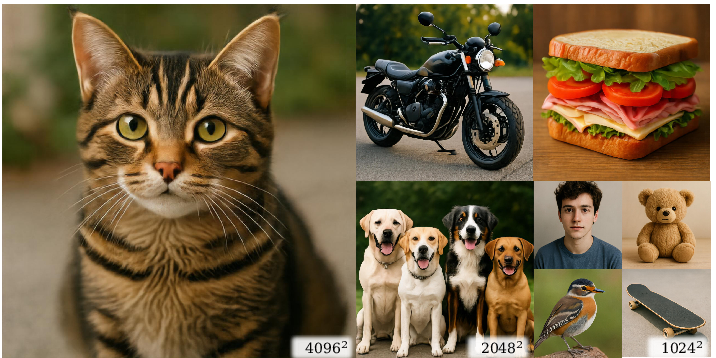
\includegraphics[height=0.43\textheight]{../project page/assets/fig_our_results.png}%
    \hspace{0.025\textwidth}%
    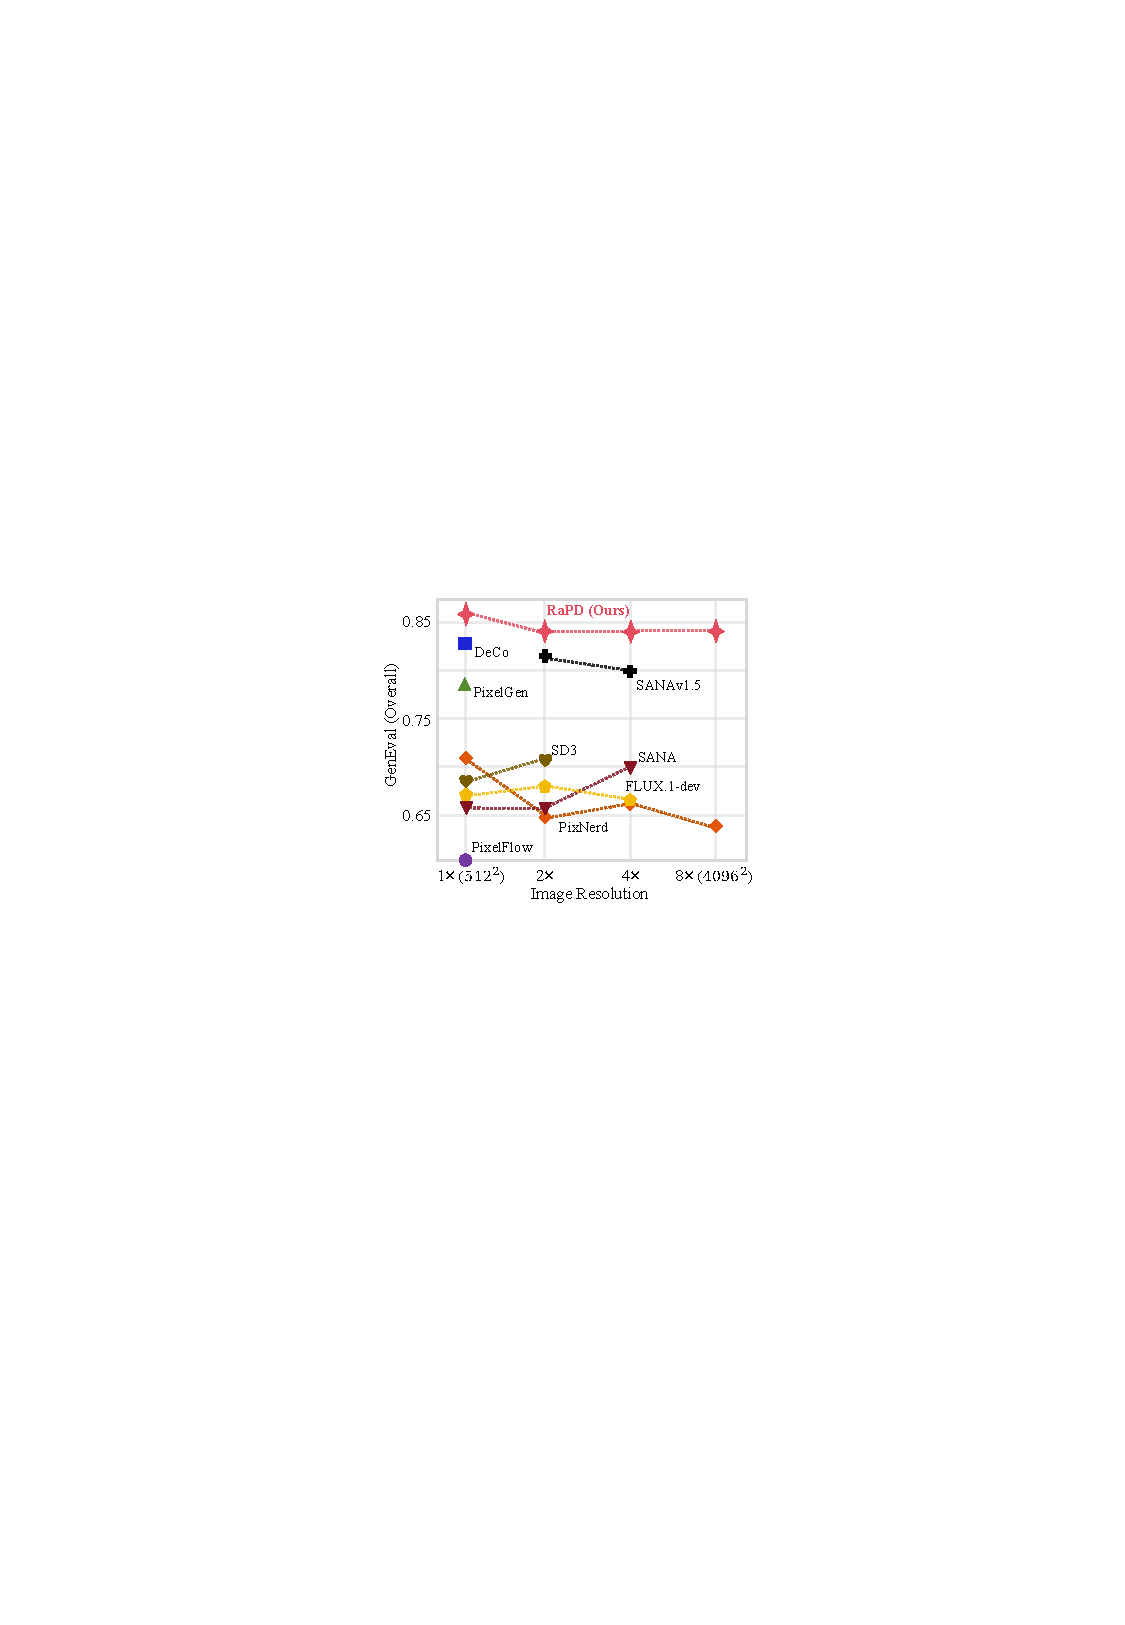
\includegraphics[height=0.43\textheight]{fig_teaser.pdf}\\[1.5em]
    
\includegraphics[width=0.8\textwidth,height=0.1\textheight,keepaspectratio]{./logo_horizon.pdf}
  \end{center}
\end{frame}

% =================== PAGE 2: MOTIVATION ==============================
\begin{frame}{Can one generated representation support \alert{different output resolutions}?}
  \story{We start by questioning a hidden assumption shared by today's image generative models.}
  \begin{columns}[T,onlytextwidth]
    \begin{column}{0.58\textwidth}
      \footnotesize
      \begin{itemize}
        \item The visual world is \hl{continuous}, but VAE-latent and pixel-token diffusion both operate on \hl{fixed spatial grids}.
        \item Higher resolution $\Rightarrow$ more tokens, more compute --- linear-to-quadratic scaling on the diffusion side.
        \item Coordinate-based decoders support flexible output sizes, but reconstruction-trained latents are not necessarily \hl{ready for generation}.
      \end{itemize}
      \vspace{0.4em}
      \begin{block}{Our question}
        \centering
        Can we learn a generation-ready representation that renders at continuous coordinates?
      \end{block}
    \end{column}
    \begin{column}{0.40\textwidth}
      \centering
      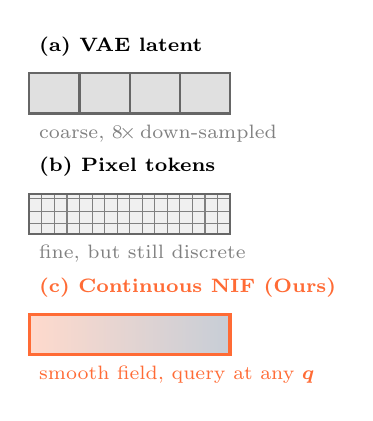
\begin{tikzpicture}[scale=0.85,every node/.style={font=\scriptsize}]
        % --- (a) VAE latent: very coarse grid ---
        \node[anchor=west] at (0,3.4) {\textbf{(a) VAE latent}};
        \fill[rapdgray!20] (0,2.4) rectangle (3.0,3.0);
        \draw[step=0.75,rapdgray,thick] (0,2.4) grid (3.0,3.0);
        \draw[rapdgray,thick] (0,2.4) rectangle (3.0,3.0);
        \node[anchor=west,gray] at (0,2.1) {coarse, $8\!\times\!$ down-sampled};
        % --- (b) Pixel tokens: fine grid ---
        \node[anchor=west] at (0,1.6) {\textbf{(b) Pixel tokens}};
        \fill[rapdgray!10] (0,0.6) rectangle (3.0,1.2);
        \draw[step=0.1875,gray,thin] (0,0.6) grid (3.0,1.2);
        \draw[rapdgray,thick] (0,0.6) rectangle (3.0,1.2);
        \node[anchor=west,gray] at (0,0.3) {fine, but still discrete};
        % --- (c) Continuous NIF: smooth gradient, no grid ---
        \node[anchor=west,rapdorange] at (0,-0.2) {\textbf{(c) Continuous NIF (Ours)}};
        \shade[left color=rapdorange!25,right color=rapdblue!25]
          (0,-1.2) rectangle (3.0,-0.6);
        \draw[rapdorange,very thick] (0,-1.2) rectangle (3.0,-0.6);
        \node[rapdorange,anchor=west] at (0,-1.5) {smooth field, query at any $\boldsymbol{q}$};
      \end{tikzpicture}
    \end{column}
  \end{columns}
\end{frame}

% =================== PAGE 3: GAP =====================================
\begin{frame}{Reconstruction-trained image fields are \alert{not automatically generation-ready}}
  \story{Applying a diffusion model to LIIF / CLIF latents exposes a reconstruction--generation gap.}
  \begin{columns}[T,onlytextwidth]
    \begin{column}{0.58\textwidth}
      \centering
      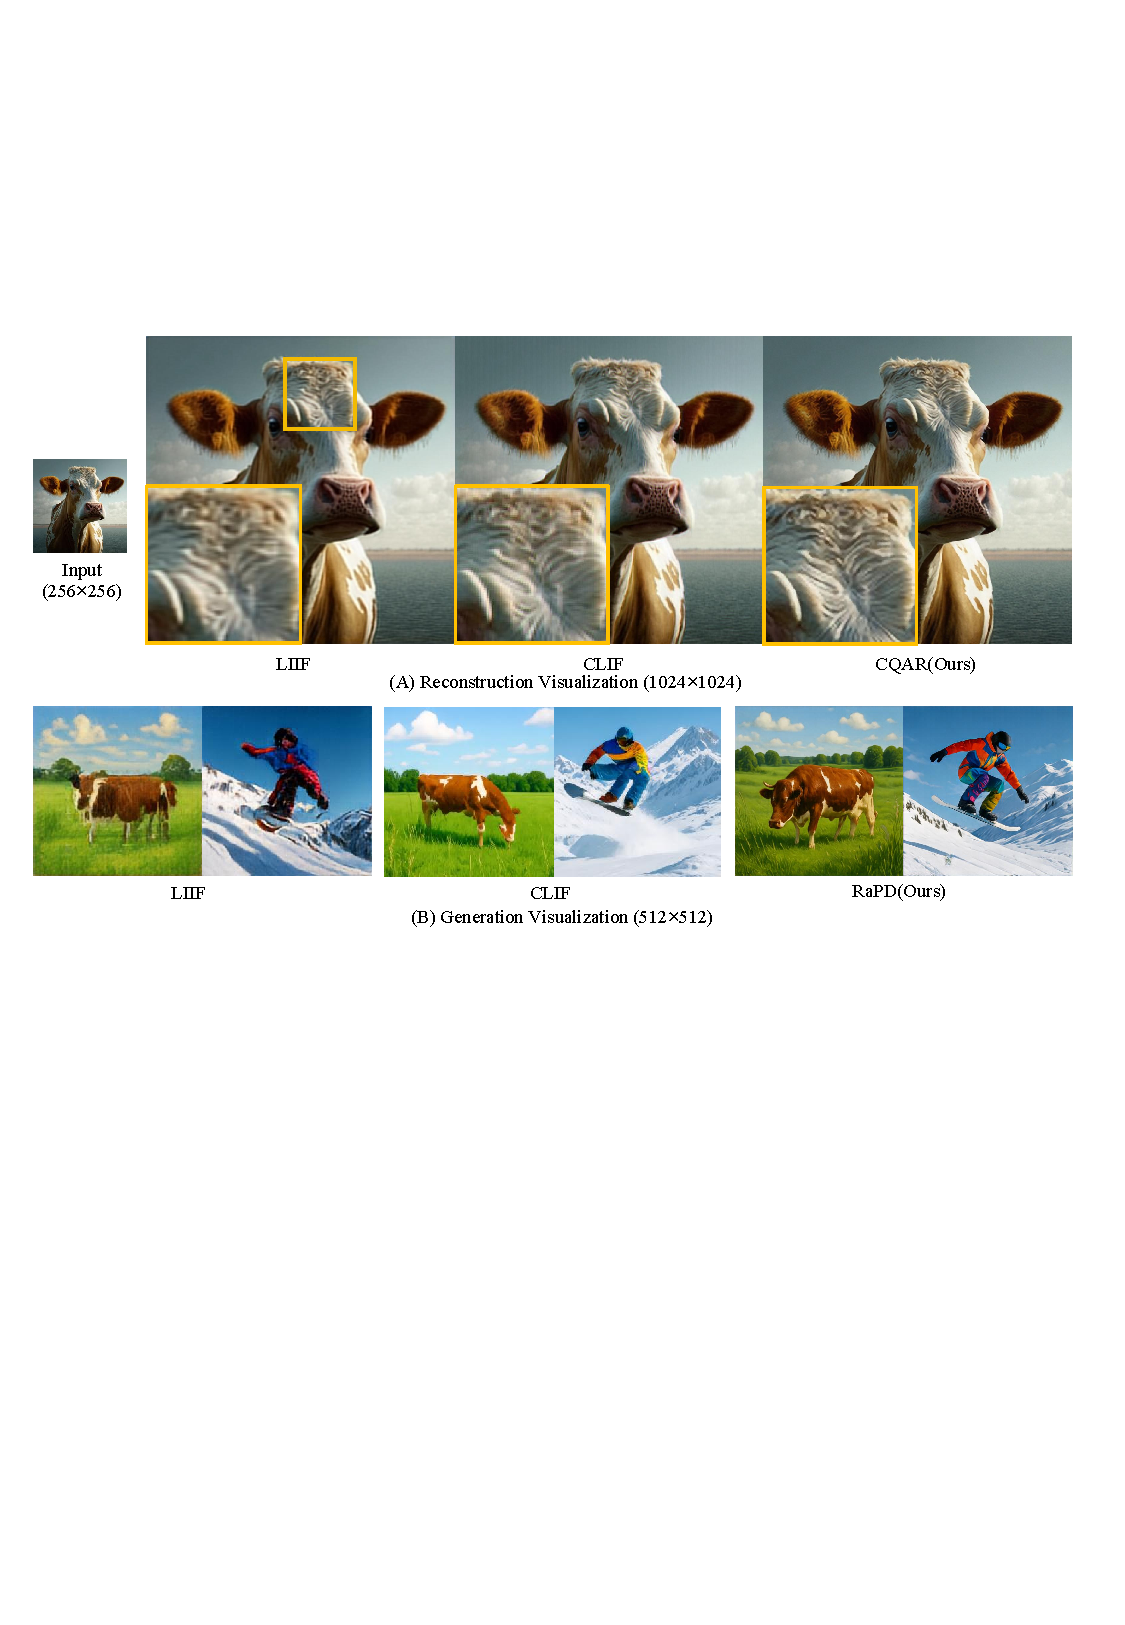
\includegraphics[width=\linewidth,height=0.55\textheight,keepaspectratio]{exp_render.pdf}\\[0.2em]
      {\scriptsize\itshape\color{rapdgray}Reconstruction--generation gap of existing NIF representations: strong super-resolution reconstruction (top) but weak text-to-image generation (bottom).}
    \end{column}
    \begin{column}{0.40\textwidth}
      \footnotesize
      \begin{itemize}
        \item LIIF / CLIF: trained for \hl{reconstruction} (pixel loss + lightweight decoder).
        \item Apply DiT-style diffusion on top $\Rightarrow$ only \hl{coarse semantics, poor visual fidelity}.
      \end{itemize}
      \vspace{0.3em}
      \begin{block}{Reconstruction--generation gap}
        \begin{itemize}
          \item Latent encodes \emph{low-level texture}, not semantic structure.
          \item Decoder is a \emph{local operator} --- no inter-pixel reasoning.
        \end{itemize}
      \end{block}
    \end{column}
  \end{columns}
\end{frame}

% =================== PAGE 4: METHOD OVERVIEW =========================
\begin{frame}{\rapd: shape the NIF (\srg) and redesign the renderer (\cqar), in \alert{two stages}}
  \story{We close the gap with two coupled innovations: SRG makes the latent generation-ready, CQAR makes the renderer semantic-aware.}
  \begin{center}
    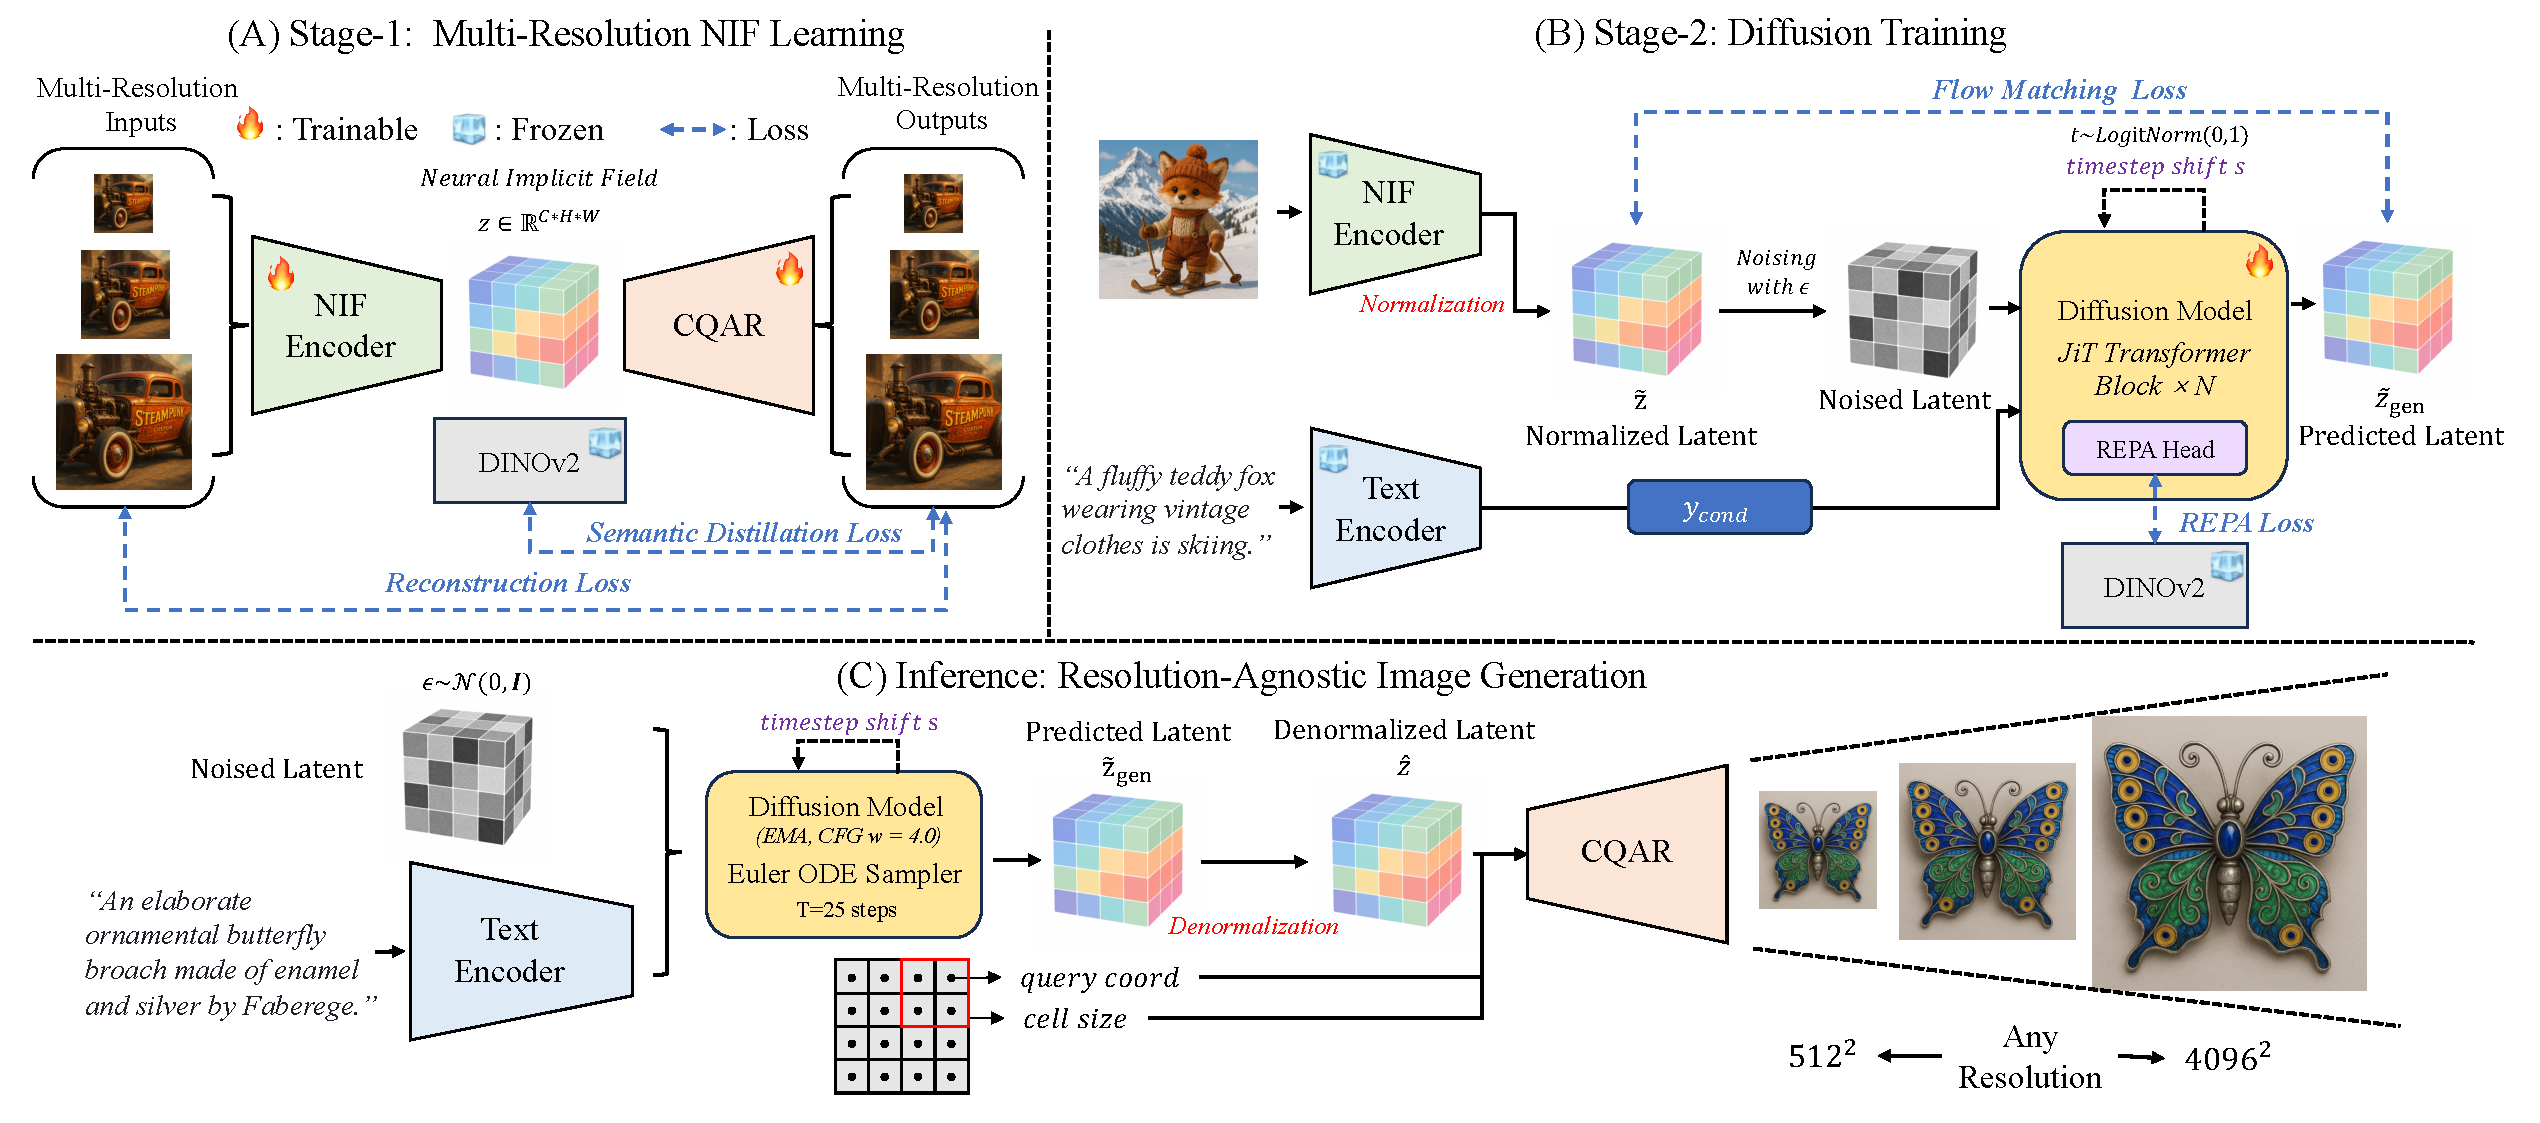
\includegraphics[width=0.92\textwidth,height=0.46\textheight,keepaspectratio]{fig1.pdf}\\[0.15em]
    {\scriptsize\itshape\color{rapdgray}Overview of RaPD. (A) Stage-1: semantically guided multi-resolution NIF learning. (B) Stage-2: text-conditioned flow matching in normalized NIF latents. (C) Inference: render one denoised latent at arbitrary resolutions via CQAR.}
  \end{center}
  \vspace{-0.2em}
  \begin{columns}[T,onlytextwidth]
    \begin{column}{0.32\textwidth}
      \footnotesize\textbf{(A) Stage-1.} NIF AE + \hl{Semantic Distillation} $\Rightarrow$ generation-aware latent.
    \end{column}
    \begin{column}{0.32\textwidth}
      \footnotesize\textbf{(B) Stage-2.} Flow matching + REPA with \hl{$s\!=\!32$} timestep shift on dense NIF latent.
    \end{column}
    \begin{column}{0.32\textwidth}
      \footnotesize\textbf{(C) Inference.} \hl{One denoised latent} $\rightarrow$ any $H'\!\times\!W'$ via the CQAR query grid.
    \end{column}
  \end{columns}
\end{frame}

% =================== PAGE 5: SRG =====================================
\begin{frame}{\srg{} turns \alert{reconstruction-oriented NIF latents} into generation-aware ones}
  \story{Innovation 1: shape the latent itself. The latent must inherit semantic structure from a vision foundation model.}
  \begin{columns}[T,onlytextwidth]
    \begin{column}{0.55\textwidth}
      \footnotesize
      \textbf{Two components:}
      \begin{itemize}
        \item \hl{Semantic Distillation}: pool $\boldsymbol{z}$ $\rightarrow$ $1\!\times\!1$ conv $\rightarrow$ align with frozen \emph{DINOv2} patch features (marginal-cosine + distance-matrix losses).
        \item \hl{Latent-Density-Aware Timestep Shift}:
          $$ t = \tfrac{t_0}{t_0+(1-t_0)\,s}, \quad s\!=\!32 $$
          (vs SD3's $s\!\in\![1,3]$); pushes mass toward noisier states where dense NIF needs most denoising.
      \end{itemize}
      \vspace{0.3em}
      \begin{block}{Why not just REPA / VA-VAE?}
        Our alignment supervises a \hl{dense NIF latent} directly, unlike prior work on downsampled VAE latents (REPA-E, VA-VAE) or denoiser features (REPA). The projection branch transfers semantic structure \hl{without changing the latent layout}, preserving the coordinate-based rendering pathway. 
      \end{block}
    \end{column}
    \begin{column}{0.43\textwidth}
      \centering
      \begin{tikzpicture}
        \node[anchor=south west, inner sep=0] (fig1) at (0,0) {%
          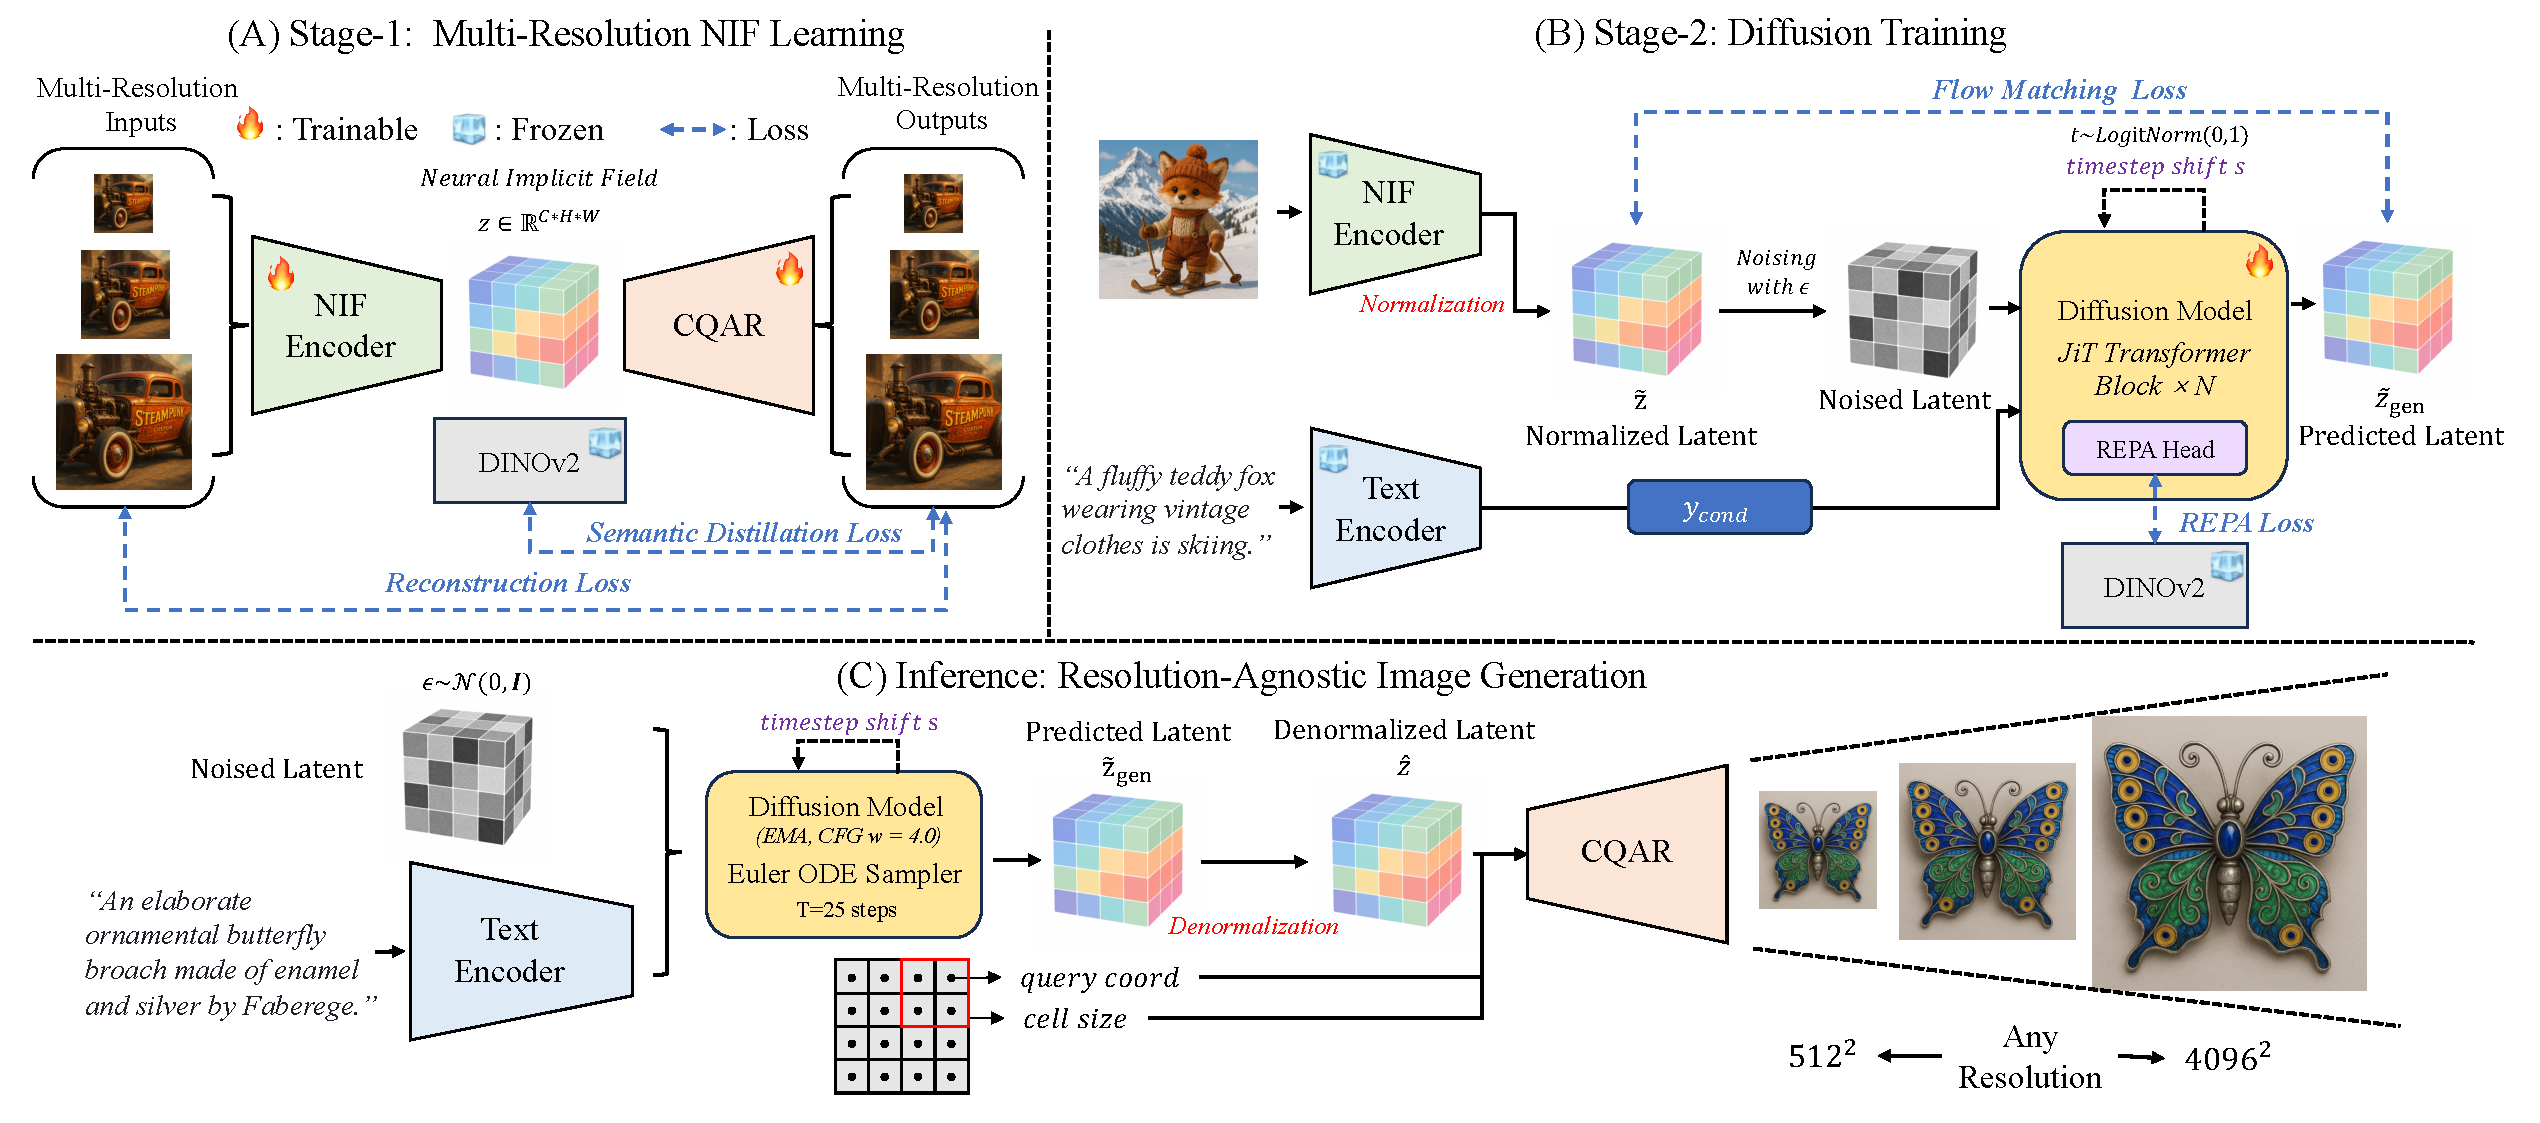
\includegraphics[width=\linewidth,height=0.62\textheight,keepaspectratio]{fig1.pdf}%
        };
        \begin{scope}[x={(fig1.south east)}, y={(fig1.north west)}]
          % --- Box 1: bottom up 10px, left edge right 20px ---
          \draw[red, dashed, very thick, rounded corners=2pt]
            (0.11, 0.535) rectangle (0.32, 0.66);
          \node[red, anchor=south, font=\scriptsize\bfseries]
            at (0.215, 0.66) {(i) Semantic Distillation};
          % --- Box 2: down another 10px, label moved above box ---
          \draw[red, dashed, very thick, rounded corners=2pt]
            (0.74, 0.80) rectangle (0.96, 0.88);
          \node[red, anchor=south, font=\scriptsize\bfseries]
            at (0.85, 0.88) {(ii) Timestep Shift};
        \end{scope}
      \end{tikzpicture}\\[0.1em]
      {\scriptsize\itshape\color{rapdgray}Two SRG components highlighted in red on the RaPD framework.}
    \end{column}
  \end{columns}
\end{frame}

% =================== PAGE 6: CQAR ====================================
\begin{frame}{\cqar{} enables \alert{inter-pixel reasoning} at decoding via coordinate-conditioned attention}
  \story{Innovation 2: redesign the renderer. A semantically rich latent is wasted if the decoder is a pure pointwise operator.}
  \begin{center}
    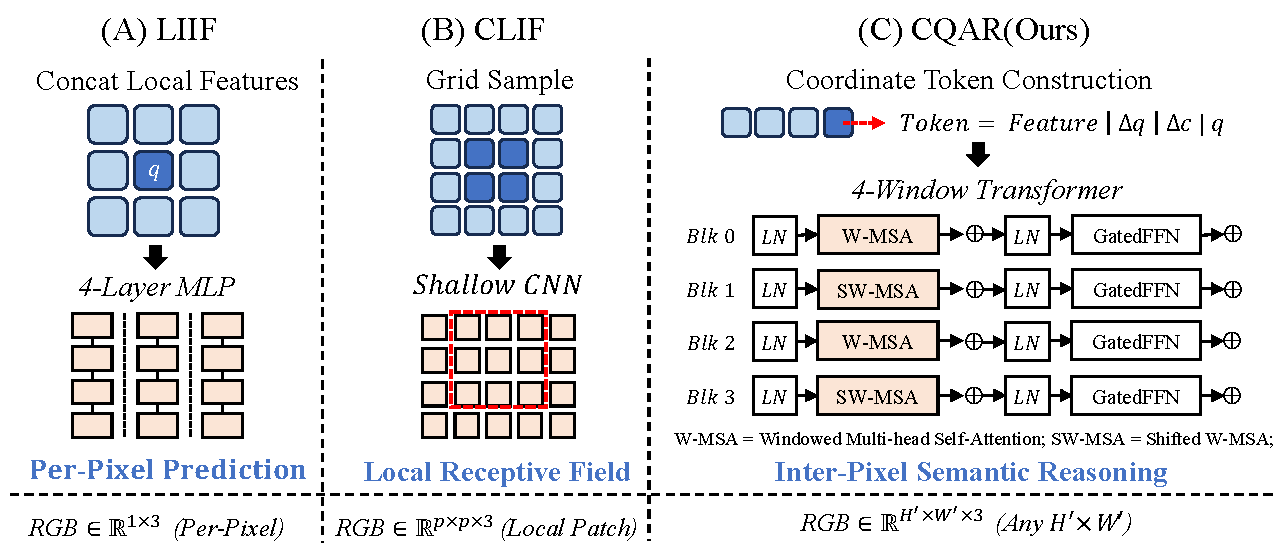
\includegraphics[width=0.85\textwidth,height=0.42\textheight,keepaspectratio]{fig2.pdf}\\[0.15em]
    {\scriptsize\itshape\color{rapdgray}Implicit decoder comparison. (A) LIIF: per-pixel MLP. (B) CLIF: shallow CNN. (C) CQAR: coordinate-conditioned windowed attention over output tokens.}
  \end{center}
  \vspace{0.1em}
  \begin{columns}[c,onlytextwidth]
    \begin{column}{0.31\textwidth}
      \centering
      \footnotesize\textbf{(A) LIIF}\\[0.15em]
      per-pixel MLP\\
      \hl{no output-token attention}
    \end{column}
    \begin{column}{0.31\textwidth}
      \centering
      \footnotesize\textbf{(B) CLIF}\\[0.15em]
      shallow CNN\\
      \hl{limited receptive field}
    \end{column}
    \begin{column}{0.31\textwidth}
      \centering
      \footnotesize\textbf{(C) CQAR (Ours)}\\[0.15em]
      windowed attention over\\
      \hl{output coordinate tokens}
    \end{column}
  \end{columns}
\end{frame}

% =================== PAGE 7: GenEval Table ===========================
\begin{frame}{Quantitative comparison on \alert{GenEval} at $512\!\times\!512$}
  \story{Progressive training ($256\rightarrow512$) reaches 0.86 overall with a 1.1B denoiser.}
  \begin{center}
  \scriptsize
  \setlength{\tabcolsep}{3pt}
  \resizebox{0.98\linewidth}{!}{%
\begin{tabular}{l|c|ccccccc}
\toprule
\multirow{2}{*}{Method} & \multirow{2}{*}{\#Params} & \multicolumn{7}{c}{GenEval $\uparrow$} \\
 &  & Single Obj. & Two Obj. & Counting & Colors & Position & Color Attr. & Overall \\
\midrule
\rowcolor{gray!15}
\multicolumn{9}{c}{$\triangledown$ \textit{Latent Diffusion Models}} \\
LDM & 1.4B & 0.92 & 0.29 & 0.23 & 0.70 & 0.02 & 0.05 & 0.37 \\
SD3 & 8B & 0.98 & 0.84 & 0.66 & 0.74 & 0.40 & 0.43 & 0.68 \\
FLUX.1-dev & 12B & 0.99 & 0.81 & 0.79 & 0.74 & 0.20 & 0.47 & 0.67 \\
SANA & 1.6B & 0.99 & 0.79 & 0.63 & 0.88 & 0.18 & 0.47 & 0.66 \\
\midrule
\rowcolor{gray!15}
\multicolumn{9}{c}{$\triangledown$ \textit{Pixel Diffusion Models}} \\
PixelFlow-XL/4 & 0.9B & -- & -- & -- & -- & -- & -- & 0.60 \\
PixNerd-XXL/16 & 1.2B & 0.97 & 0.86 & 0.44 & 0.83 & 0.71 & 0.53 & 0.73 \\
DeCo-XXL/16 & 1.1B & \textbf{1.00} & 0.92 & 0.72 & 0.91 & \textbf{0.80} & \textbf{0.79} & \textbf{0.86} \\
PixelGen-XXL/16 & 1.1B & 0.99 & 0.88 & 0.59 & 0.90 & 0.70 & 0.70 & 0.79 \\
PixNerd-XXL/16 ($\ddagger$) & 1.2B & 0.98 & 0.82 & 0.43 & 0.81 & 0.66 & 0.55 & 0.71 \\
DeCo-XXL/16 ($\ddagger$) & 1.1B & 0.99 & 0.92 & 0.65 & 0.91 & 0.71 & 0.77 & 0.83 \\
PixelGen-XXL/16 ($\ddagger$) & 1.1B & 0.99 & 0.88 & 0.58 & 0.91 & 0.70 & 0.67 & 0.79 \\
\midrule
\textbf{RaPD} & 1.1B & \underline{0.99} & \textbf{0.93} & \underline{0.72} & \textbf{0.93} & 0.77 & 0.74 & \underline{0.85} \\
\textbf{RaPD (256$\rightarrow$512)} & 1.1B & \underline{0.99} & \textbf{0.93} & \textbf{0.77} & \underline{0.92} & \underline{0.79} & \underline{0.78} & \textbf{0.86} \\
\bottomrule
\end{tabular}
}\\[0.4em]
  {\scriptsize\itshape\color{rapdgray}Text-to-image generation on GenEval at a $512\!\times\!512$ resolution. $\ddagger$ denotes results obtained by running the officially released models with the same random seed and computing environment as RaPD.}
  \end{center}
\end{frame}

% =================== PAGE 8: DPG-Bench Table =========================
\begin{frame}{Quantitative comparison on \alert{DPG-Bench} at $512\!\times\!512$}
  \story{Progressive training reaches 82.9, above the reproduced pixel-diffusion baselines.}
  \begin{center}
  \scriptsize
  \setlength{\tabcolsep}{4pt}
  \resizebox{0.98\linewidth}{!}{%
\begin{tabular}{l|c|cccccc}
\toprule
\multirow{2}{*}{Method} & \multirow{2}{*}{\#Params} & \multicolumn{6}{c}{{DPG-Bench} $\uparrow$}  \\
 &  & Global & Entity & Attribute & Relation & Other & Average \\
\midrule
\rowcolor{gray!15}
\multicolumn{8}{c}{$\triangledown$ \textit{Latent Diffusion Models}} \\
SD v2 & 0.9B & 77.7 & 78.1 & 74.9 & 80.7 & 80.7 & 68.1 \\
PixArt-$\alpha$ & 0.6B & 75.0 & 79.3 & 78.6 & 82.6 & 77.0 & 71.1 \\
SANA & 1.6B & 90.3 & 91.2 & 89.0 & 88.9 & 92.0 & 85.5 \\
\midrule
\rowcolor{gray!15}
\multicolumn{8}{c}{$\triangledown$ \textit{Pixel Diffusion Models}} \\
PixelFlow-XL/4 & 0.9B & -- & -- & -- & -- & -- & 77.9 \\
PixNerd-XXL/16 & 1.2B & 80.5 & 87.9 & 87.2 & \textbf{91.3} & 72.8 & 80.9 \\
DeCo-XXL/16 & 1.1B & -- & -- & -- & -- & -- & 81.4 \\
PixNerd-XXL/16 ($\ddagger$) & 1.2B & 87.2 & 87.1 & 88.9 & 87.1 & \textbf{89.8} & 81.5 \\
PixelGen-XXL/16 ($\ddagger$) & 1.1B & 81.4 & 88.8 & 86.7 & 88.9 & 88.9 & 80.4 \\
DeCo-XXL/16 ($\ddagger$) & 1.1B & \textbf{88.6} & 88.4 & 88.9 & 87.6 & 86.0 & 81.2 \\
\midrule
\textbf{RaPD} & 1.1B & 85.1 & 87.7 & \underline{88.9} & \underline{89.6} & 84.1 & \underline{81.6} \\
\textbf{RaPD (256$\rightarrow$512)} & 1.1B & 81.3 & \textbf{89.9} & \textbf{89.7} & 88.9 & 81.2 & \textbf{82.9} \\
\bottomrule
\end{tabular}
}\\[0.4em]
  {\scriptsize\itshape\color{rapdgray}Text-to-image generation results on DPG-Bench at a $512\!\times\!512$ resolution. $\ddagger$ denotes results obtained by running the officially released models with the same random seed and computing environment as RaPD.}
  \end{center}
\end{frame}

% =================== PAGE 9: QUALITATIVE COMPARISON ==================
\begin{frame}{Qualitative comparison: \alert{visual fidelity} and prompt adherence}
  \story{Side-by-side with the closest pixel-diffusion baselines on the same prompts.}
  \begin{center}
    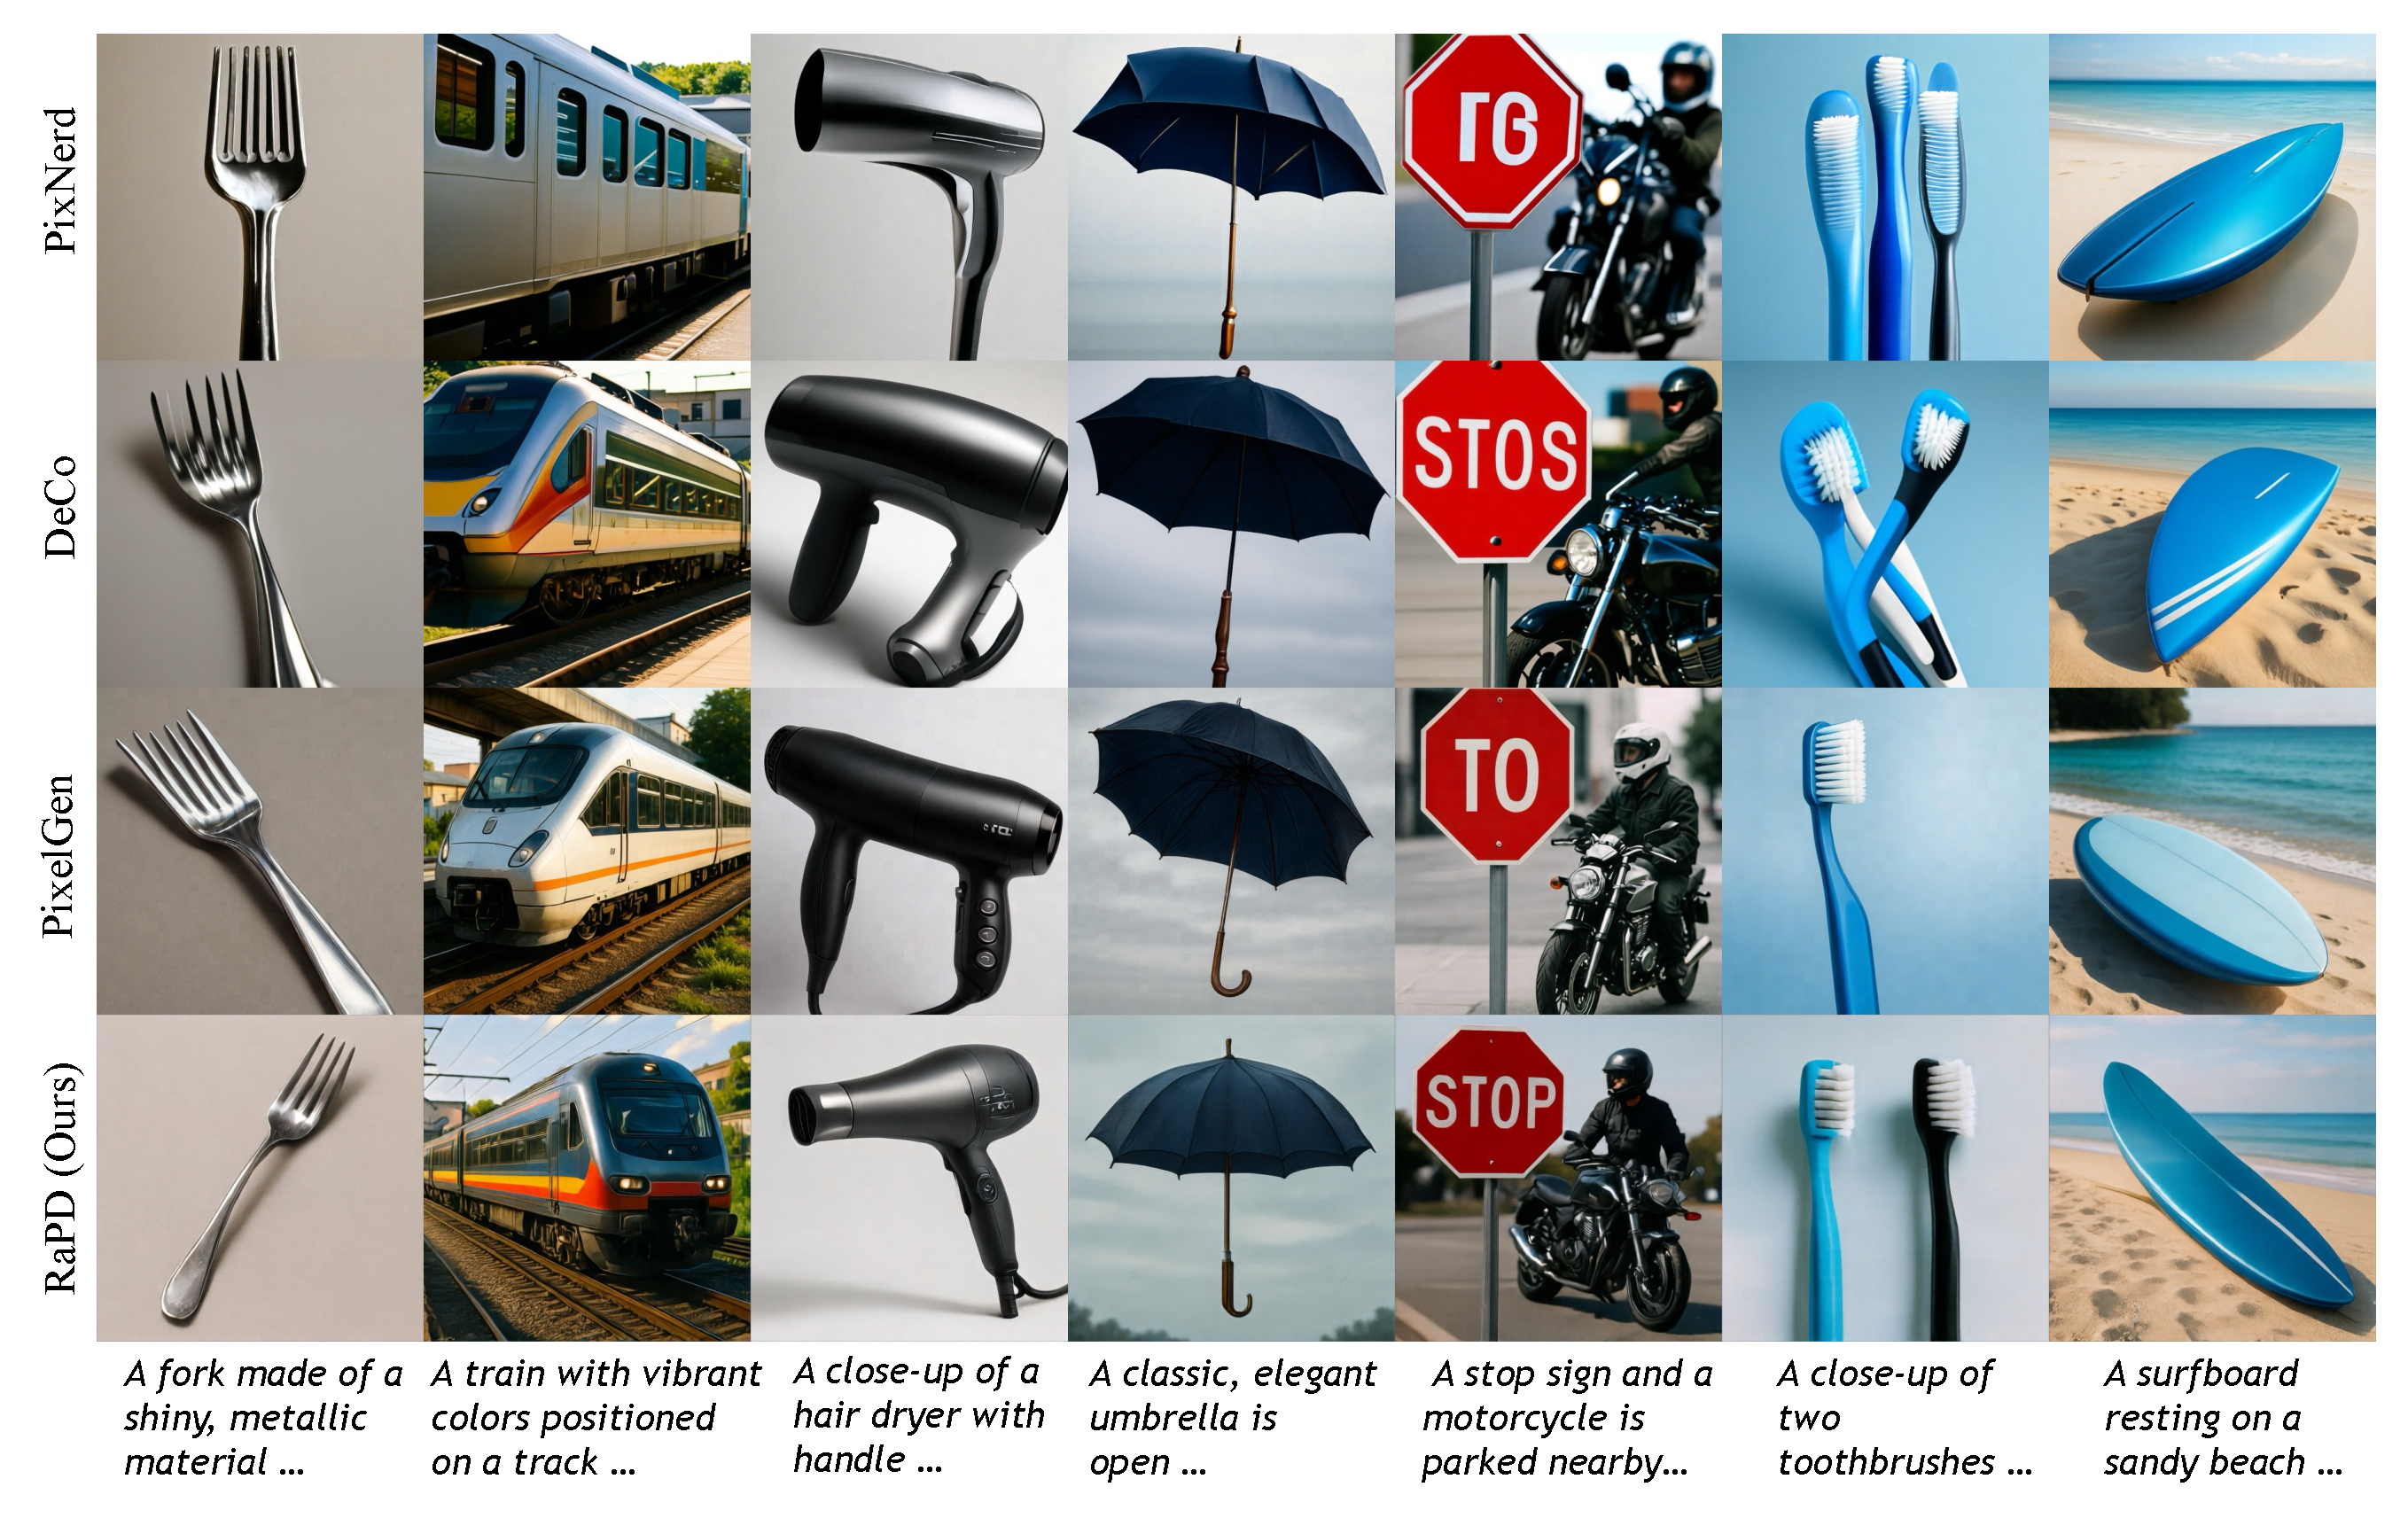
\includegraphics[width=0.96\textwidth,height=0.70\textheight,keepaspectratio]{fig_comparison.pdf}\\[0.15em]
    {\scriptsize\itshape\color{rapdgray}Qualitative text-to-image comparison with baselines (PixelGen, DeCo, PixNerd) at $512^2$.}
  \end{center}
\end{frame}

% =================== PAGE 10: ARBITRARY-RESOLUTION ===================
\begin{frame}{Fixed latent $\to$ \alert{Any Resolution}: GenEval and DPG-Bench across scales}
  \story{Same model and same denoised latent; only the CQAR query coordinate grid changes.}
  \begin{center}
    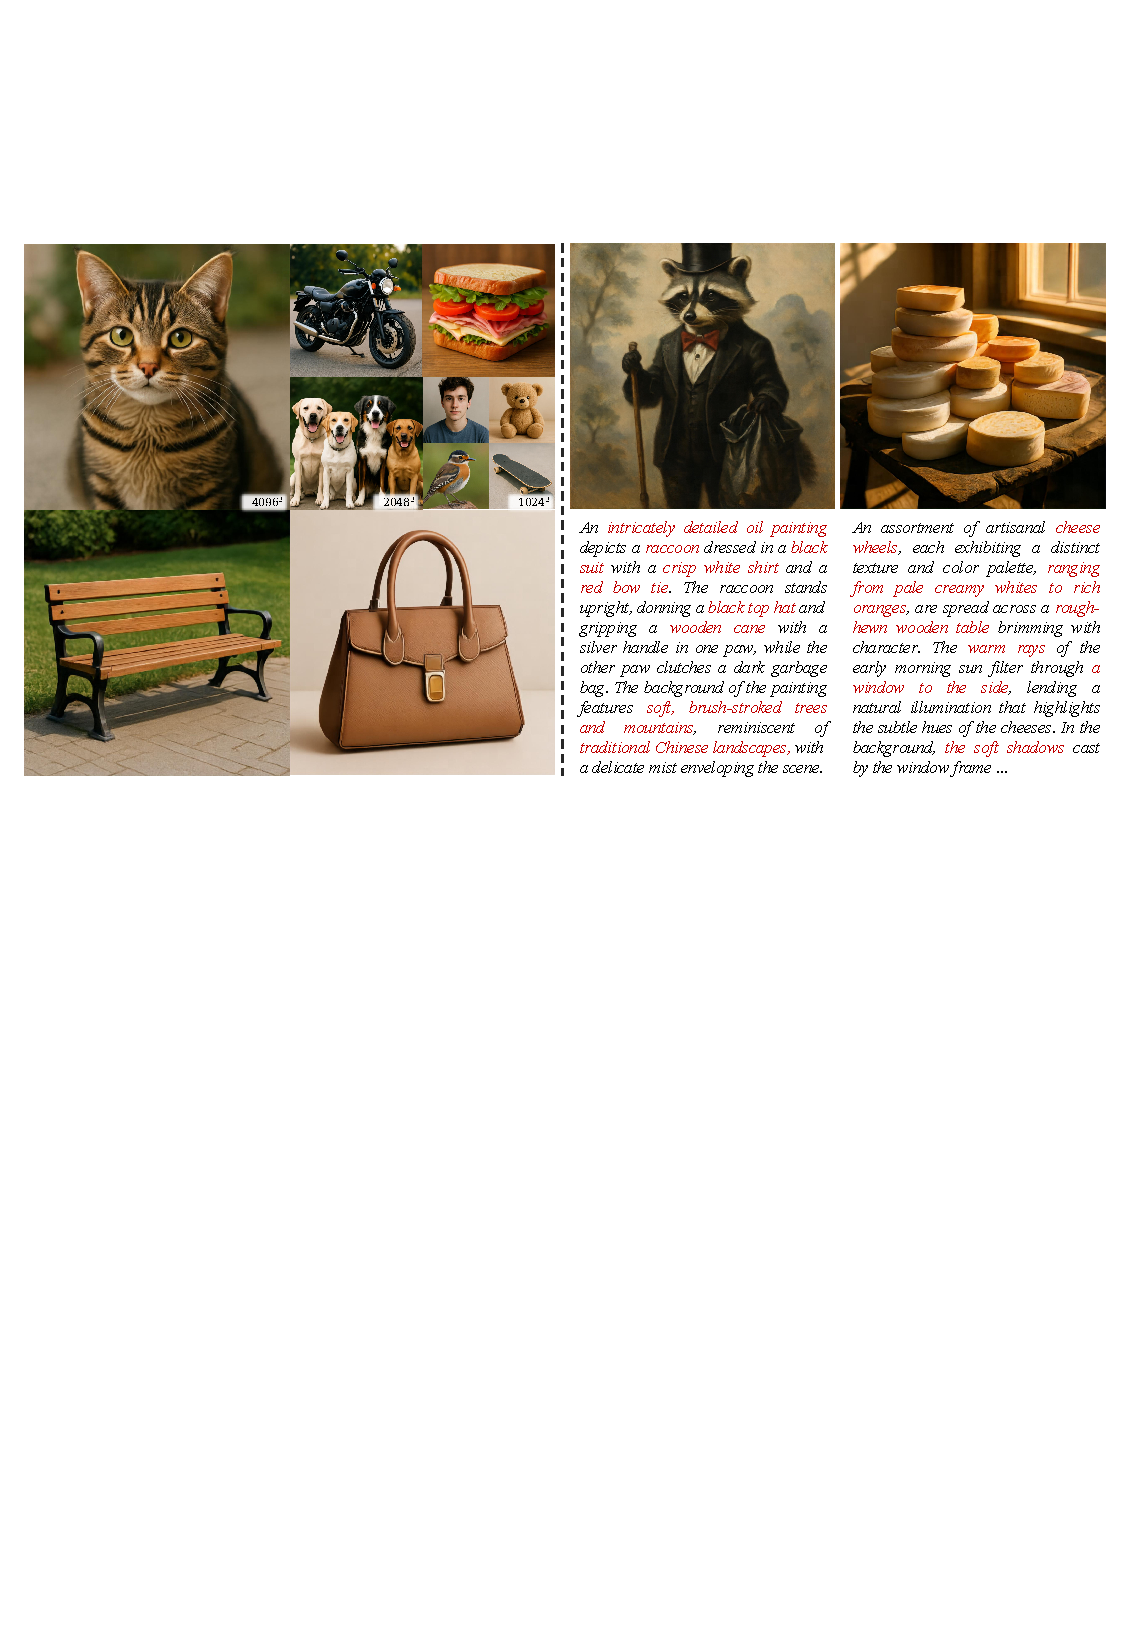
\includegraphics[width=0.92\textwidth,height=0.70\textheight,keepaspectratio]{fig_our_results.pdf}
  \end{center}
  \vspace{-0.4em}
  \hspace*{0.04\textwidth}%
  \begin{minipage}{0.92\textwidth}
    \raggedright
    \scriptsize\itshape\color{rapdgray}
    (A) Results on GenEval: samples generated from short, compositional prompts and rendered at multiple output resolutions;\\
    (B) Results on DPG-Bench: RaPD faithfully captures fine-grained semantic and stylistic details specified in the prompt.
  \end{minipage}
\end{frame}


% Camera-ready addition: progressive high-resolution training.
\begin{frame}{High-resolution generation: strong composition, remaining prompt-detail gap}
  \story{Evaluate the progressively trained $256\rightarrow1024$ model at matched output resolutions.}
  \begin{center}
  \small
  \begin{tabular}{lccccc}
  \toprule
  & & \multicolumn{2}{c}{$1024^2$} & \multicolumn{2}{c}{$2048^2$} \\
  Method & Params & GenEval $\uparrow$ & DPG $\uparrow$ & GenEval $\uparrow$ & DPG $\uparrow$ \\
  \midrule
  SANA & 1.6B & 0.66 & 84.8 & 0.70 & 83.1 \\
  SANA-v1.5 & 1.6B & 0.82 & 84.5 & 0.80 & 83.8 \\
  FLUX.1-dev & 12B & 0.68 & 83.1 & 0.66 & 82.8 \\
  \rowcolor{lightbluepurple}
  RaPD ($256\rightarrow1024$) & 1.1B & \textbf{0.85} & 80.3 & \textbf{0.85} & 80.1 \\
  \bottomrule
  \end{tabular}
  \end{center}
  \begin{itemize}
    \item Best GenEval among these methods at both evaluated resolutions.
    \item $2048^2$ is beyond the $1024^2$ training supervision range.
    \item Lower DPG scores show room to improve detailed prompt adherence.
  \end{itemize}
\end{frame}

\begin{frame}{Training setup and the role of semantic supervision}
  \story{Stage-1 latent distillation and Stage-2 denoiser alignment play complementary roles.}
  \begin{columns}[T,onlytextwidth]
  \begin{column}{0.47\textwidth}
  \footnotesize
  \begin{itemize}
    \item Data: approximately 36M BLIP3o images; 60k curated images for fine-tuning.
    \item Stage-1: train the encoder and renderer for 10k steps with semantic distillation.
    \item Stage-2: freeze the encoder and renderer; train the denoiser with flow matching and REPA feature alignment.
    \item Sampling: 25 Euler steps, classifier-free guidance scale 4.0.
  \end{itemize}
  \end{column}
  \begin{column}{0.51\textwidth}
  \scriptsize
  \begin{tabular}{lcc}
  \toprule
  Setting & GenEval & DPG \\
  \midrule
  No Stage-1 distillation & 0.83 & 78.9 \\
  No Stage-2 REPA & 0.61 & 56.6 \\
  \rowcolor{lightbluepurple}
  Full model & \textbf{0.85} & \textbf{81.6} \\
  \bottomrule
  \end{tabular}
  \vspace{1em}
  \begin{block}{Interpretation}
  Removing REPA gives the largest drop under the same training budget. Stage-1 distillation provides further gains. These ablations use the base RaPD model, not the progressive-training variant.
  \end{block}
  \end{column}
  \end{columns}
\end{frame}
% =================== PAGE 11: COMPUTE SCALING TABLE ==================
\begin{frame}{Efficiency: \alert{Diffusion cost stays fixed} as output resolution grows}
  \story{Increasing output size leaves RaPD's denoising token count unchanged; rendering still adds cost.}
  \vspace{0.5em}
  \begin{center}
  \scriptsize
  \setlength{\tabcolsep}{4pt}
  \begin{tabular}{l|cc|cc|cc|cc}
    \toprule
    \multirow{2}{*}{Method} &
    \multicolumn{2}{c|}{$512\!\times\!512$} &
    \multicolumn{2}{c|}{$1024\!\times\!1024$} &
    \multicolumn{2}{c|}{$2048\!\times\!2048$} &
    \multicolumn{2}{c}{$4096\!\times\!4096$} \\
     &
    \#Tokens & Time (s) &
    \#Tokens & Time (s) &
    \#Tokens & Time (s) &
    \#Tokens & Time (s) \\
    \midrule
    PixelGen        & 1{,}024 & 0.19 & 4{,}096  & 0.60 & 16{,}384 & 4.72 & 65{,}536 & 61.46 \textcolor{red}{(+61.27)} \\
    DeCo            & 1{,}024 & 0.21 & 4{,}096  & 0.67 & 16{,}384 & 5.03 & 65{,}536 & 62.72 \textcolor{red}{(+62.51)} \\
    \rowcolor{lightbluepurple}
    \textbf{RaPD}   & 1{,}024 & 0.23 & 1{,}024  & 0.34 & 1{,}024  & 0.68 & 1{,}024  & \textbf{2.13} {\color{rapdorange}(+1.9)} \\
    \bottomrule
  \end{tabular}\\[0.4em]
  {\scriptsize\itshape\color{rapdgray}Computational scaling with output resolution. Per-image inference time on an NVIDIA B200 GPU is reported at $1\!\times\!$ to $8\!\times\!$ output scales. RaPD keeps the expensive denoising stage nearly fixed, while fixed-grid pixel diffusion methods grow with the output resolution.}
  \end{center}
  \vspace{0.5em}
  \begin{block}{Take-away}
    \centering
    \hl{Diffusion cost} is fixed regardless of output size.
    Only \hl{CQAR rendering} grows linearly with the queried output token count.
  \end{block}
\end{frame}

% =================== PAGE 12: ABLATIONS ==============================
\begin{frame}{Ablation Study: Each Component is Necessary}
  \story{The paper studies semantic supervision, timestep shift, and coordinate-based rendering.}
  \begin{columns}[T,onlytextwidth]
    \begin{column}{0.48\textwidth}
      \centering
      % Fixed-height image box: keeps figure visually anchored regardless of aspect ratio
      \parbox[t][0.54\textheight][t]{\linewidth}{%
        \centering
        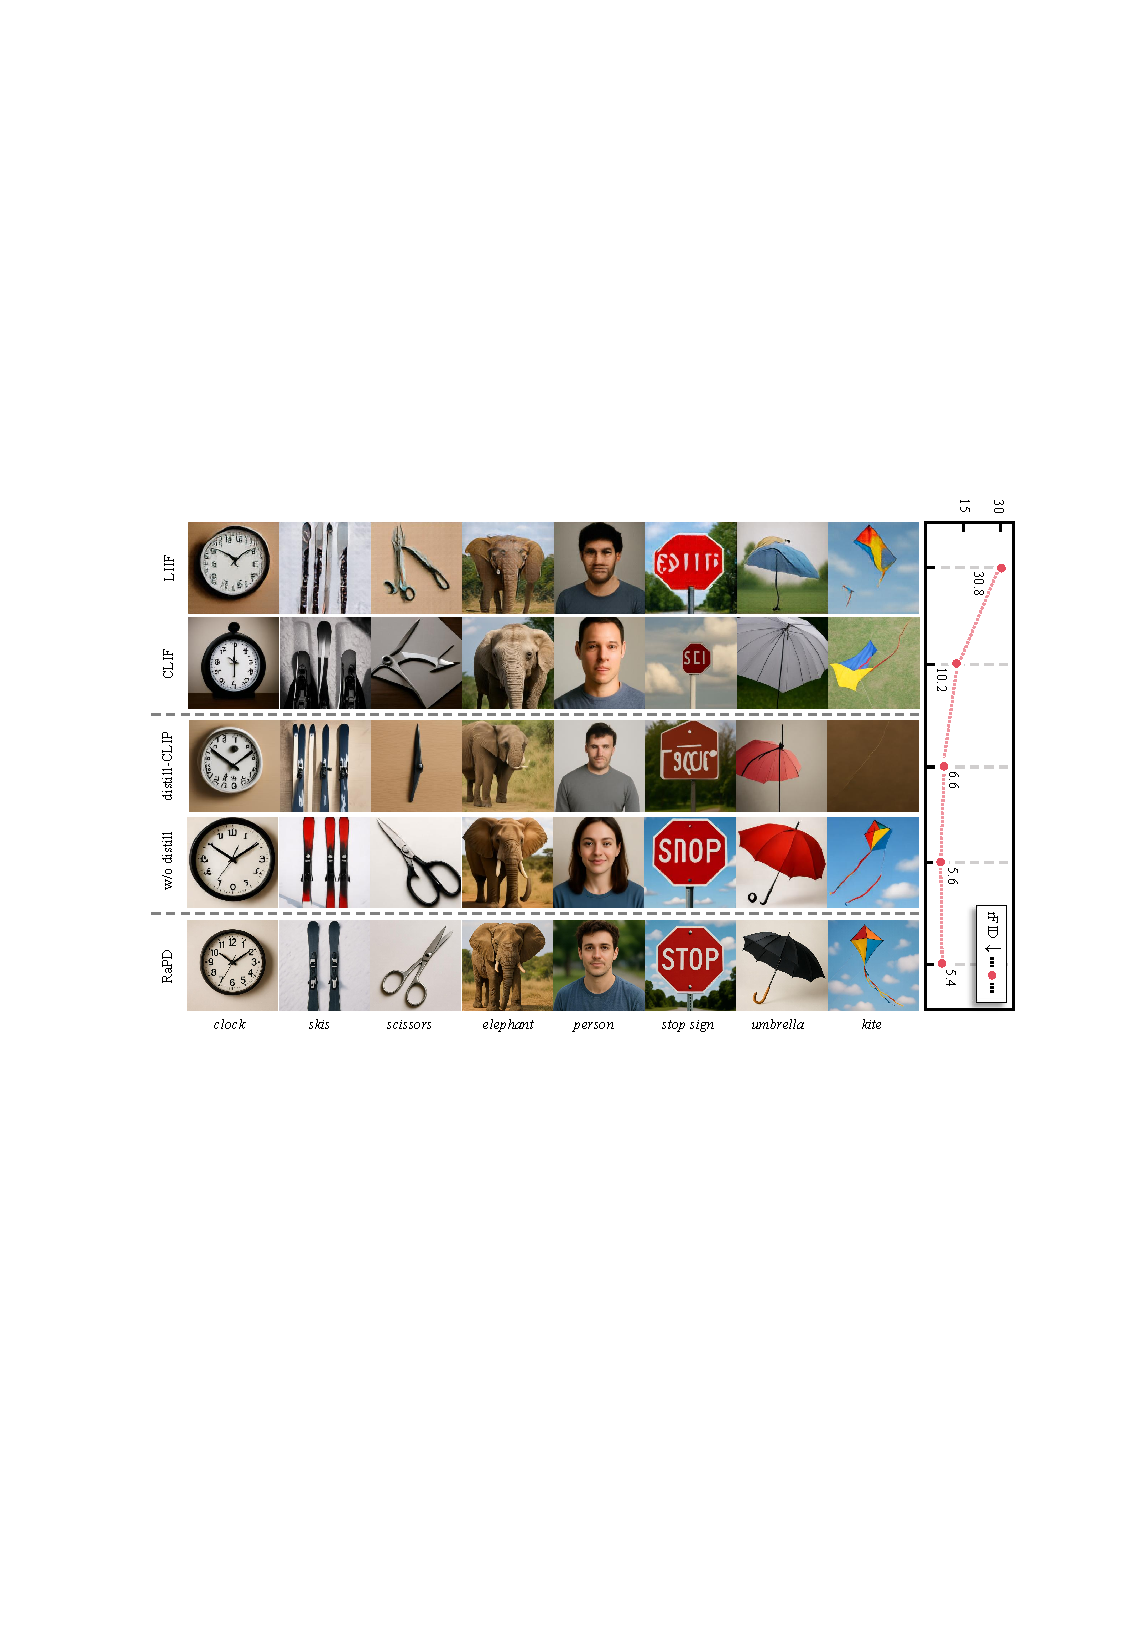
\includegraphics[width=1.28\linewidth,height=0.52\textheight,keepaspectratio]{exp_ablation.pdf}%
      }\\[0.4em]
      {\scriptsize\itshape\color{rapdgray}Ablation study of representation alignment and CQAR.}\\[0.4em]
      {\scriptsize \textbf{(a) Semantic supervision}:\\distillation and renderer ablations}
    \end{column}
    \begin{column}{0.48\textwidth}
      \centering
      \parbox[t][0.54\textheight][t]{\linewidth}{%
        \centering
        \vspace*{0.05\textheight}
        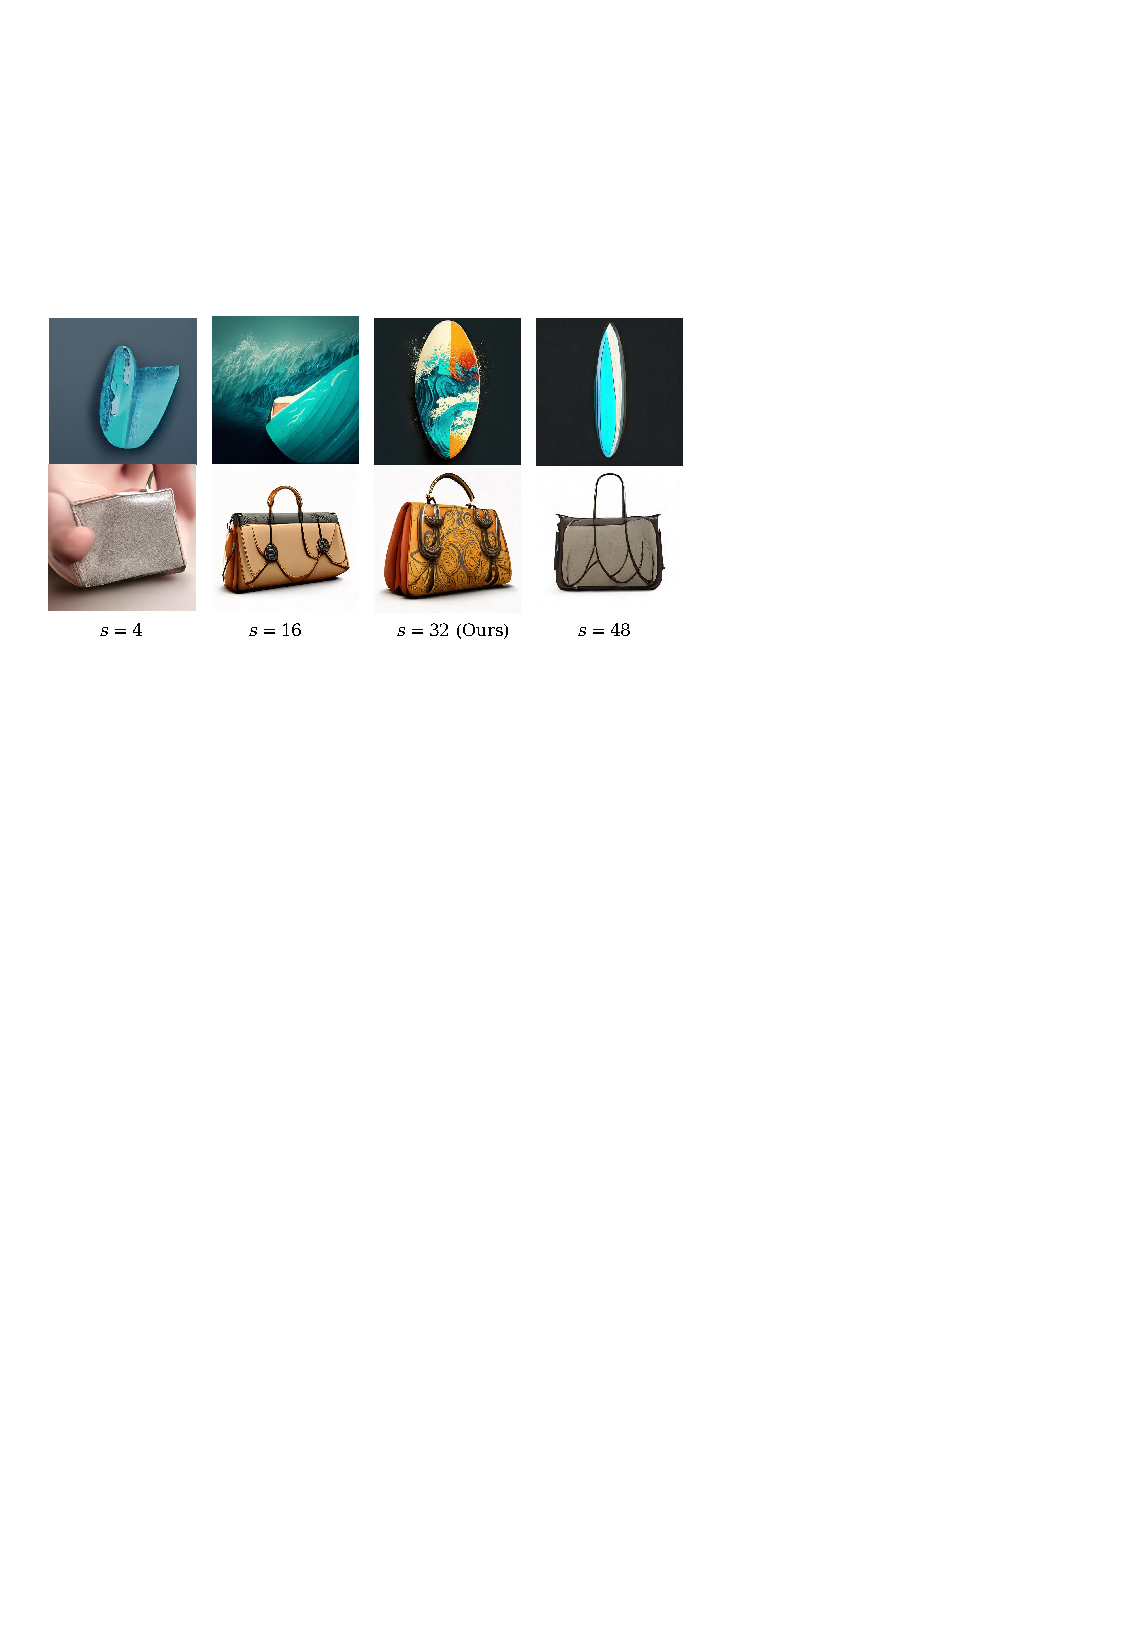
\includegraphics[width=\linewidth,height=0.40\textheight,keepaspectratio]{exp_timeshift.pdf}%
      }\\[0.4em]
      {\scriptsize\itshape\color{rapdgray}Effect of timestep shift on a test prompt.}\\[0.4em]
      {\scriptsize \textbf{(b) Timestep shift}: small $s$ degrades\\structure; $s\!=\!32$ best}
    \end{column}
    
  \end{columns}
\end{frame}

% =================== PAGE 13: CONCLUSION =============================
\begin{frame}{Conclusions: Contributions, Limitations, and Future work}
  \story{We end with an honest summary: what we have shown, where the boundaries lie, and what comes next.}

  % --- Contributions banner (top, compact) ---
  \begin{block}{Contributions}
    \scriptsize
    \begin{itemize}[label=$\bullet$,leftmargin=1.4em,topsep=0pt,itemsep=2pt,parsep=0pt]
      \item \textbf{(i) \rapd:} a resolution-agnostic pixel diffusion framework that directly generates continuous image signals in a NIF latent space.
      \item \textbf{(ii) \srg:} transforms reconstruction-oriented continuous latents into generation-aware representations via semantic distillation + density-aware timestep shift.
      \item \textbf{(iii) \cqar:} coordinate-conditioned, scale-aware Transformer renderer for spatially coherent, arbitrary-resolution rendering with fixed diffusion cost.
    \end{itemize}
  \end{block}
  \vspace{0.2em}

  % --- Limitations + Future Work (2 columns) ---
  \begin{columns}[T,onlytextwidth]
    \begin{column}{0.49\textwidth}
      \begin{block}{Limitations}
        \scriptsize
        \begin{itemize}[label=$\bullet$,leftmargin=1.2em,topsep=0pt,itemsep=2pt,parsep=0pt]
          \item Training data scale (36M; vs commercial billion-scale).
          \item Compact text encoder (Qwen3-1.7B).
          \item Inference stack not yet hardware-optimized.
        \end{itemize}
      \end{block}
    \end{column}
    \begin{column}{0.49\textwidth}
      \begin{block}{Future Work}
        \scriptsize
        \begin{itemize}[label=$\bullet$,leftmargin=1.2em,topsep=0pt,itemsep=2pt,parsep=0pt]
          \item Scale training data and denoiser capacity.
          \item Editing \& control (ControlNet, instruction editing).
          \item Hardware-aware inference (FlashAttention, FP8, fused kernels).
        \end{itemize}
      \end{block}
    \end{column}
  \end{columns}
  \vspace{0.3em}
  \begin{center}
    \scriptsize\color{rapdgray}\itshape Paper: \href{https://arxiv.org/abs/2605.15908}{arxiv.org/abs/2605.15908} \quad Paper ID: 5904
  \end{center}
\end{frame}

% =====================================================================
\end{document}
